% Name: Composition and tensor product
% Description: Boxes stacked on one wire compose; boxes side by side are tensored.
% Tags: composition, tensor product, monoidal category

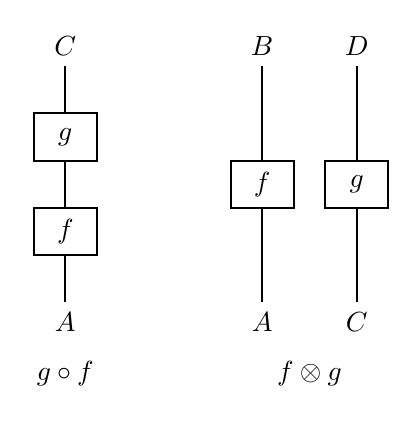
\begin{tikzpicture}[thick, box/.style={draw, fill=white, minimum width=8mm, minimum height=6mm}]
  \draw (0,0) node[below] {$A$} -- (0,3) node[above] {$C$};
  \node[box] at (0,0.9) {$f$};
  \node[box] at (0,2.1) {$g$};
  \node at (0,-0.9) {$g \circ f$};

  \draw (2.5,0) node[below] {$A$} -- (2.5,3) node[above] {$B$};
  \draw (3.7,0) node[below] {$C$} -- (3.7,3) node[above] {$D$};
  \node[box] at (2.5,1.5) {$f$};
  \node[box] at (3.7,1.5) {$g$};
  \node at (3.1,-0.9) {$f \otimes g$};
\end{tikzpicture}
